\documentclass{article}

% Recommended, but optional, packages for figures and better typesetting:
\usepackage{microtype}
\usepackage{graphicx}
% TODO figure out why we must comment this out with subcaption
%\usepackage{subfigure}
\usepackage{booktabs} % for professional tables

\usepackage[hyphens]{url}            % simple URL typesetting
\usepackage{amsmath}
\usepackage{amsfonts}       % blackboard math symbols
\usepackage{nicefrac}       % compact symbols for 1/2, etc.
\usepackage{subcaption}
\usepackage[group-separator={,}]{siunitx}
\usepackage{placeins}

% hyperref makes hyperlinks in the resulting PDF.
% If your build breaks (sometimes temporarily if a hyperlink spans a page)
% please comment out the following usepackage line and replace
% \usepackage{icml2019} with \usepackage[nohyperref]{icml2019} above.
\usepackage{hyperref}

% Attempt to make hyperref and algorithmic work together better:
\newcommand{\theHalgorithm}{\arabic{algorithm}}

% Use the following line for the initial blind version submitted for review:
\usepackage{icml2019}

% If accepted, instead use the following line for the camera-ready submission:
%\usepackage[accepted]{icml2019}

% The \icmltitle you define below is probably too long as a header.
% Therefore, a short form for the running title is supplied here:
\icmltitlerunning{Metropolis-Hastings Generative Adversarial Networks: Supplementary Material}

\newcommand{\exfactor}{1.0}

\begin{document}

\twocolumn[
\icmltitle{Metropolis-Hastings Generative Adversarial Networks\\Supplementary Material}

% It is OKAY to include author information, even for blind
% submissions: the style file will automatically remove it for you
% unless you've provided the [accepted] option to the icml2019
% package.

% List of affiliations: The first argument should be a (short)
% identifier you will use later to specify author affiliations
% Academic affiliations should list Department, University, City, Region, Country
% Industry affiliations should list Company, City, Region, Country

% You can specify symbols, otherwise they are numbered in order.
% Ideally, you should not use this facility. Affiliations will be numbered
% in order of appearance and this is the preferred way.
\icmlsetsymbol{equal}{*}

\begin{icmlauthorlist}
\icmlauthor{Ryan Turner}{uber}
\icmlauthor{Jane Hung}{uber}
\icmlauthor{Yunus Saatci}{uber}
\icmlauthor{Jason Yosinski}{uber}
\end{icmlauthorlist}

\icmlaffiliation{uber}{Uber AI Labs}

\icmlcorrespondingauthor{Ryan Turner}{ryan.turner@uber.com}

% You may provide any keywords that you
% find helpful for describing your paper; these are used to populate
% the "keywords" metadata in the PDF but will not be shown in the document
% TODO
\icmlkeywords{Machine Learning, ICML}

\vskip 0.3in
]

\begin{figure}[htbp]
    \centering
    \begin{subfigure}[b]{0.49\textwidth}
       \centering
       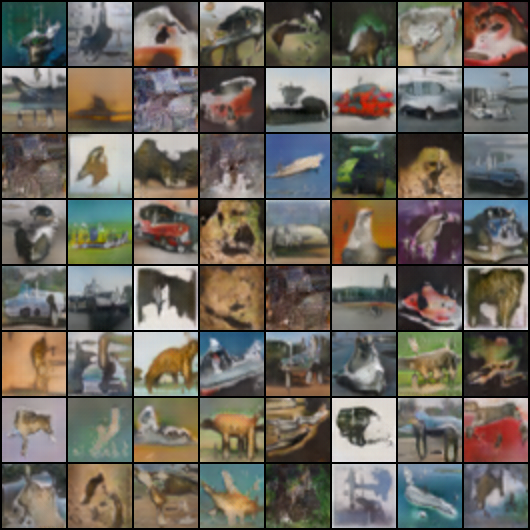
\includegraphics[width=1.0\textwidth]{figures/cifar/192_base_raw_base.png}
       \caption{GAN}
    \end{subfigure}
    \begin{subfigure}[b]{0.49\textwidth}
       \centering
       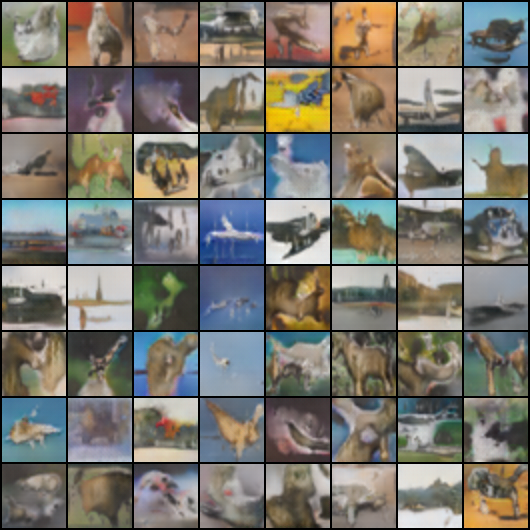
\includegraphics[width=1.0\textwidth]{figures/cifar/192_base_raw_reject.png}
       \caption{DRS}
    \end{subfigure}
    \begin{subfigure}[b]{0.49\textwidth}
       \centering
       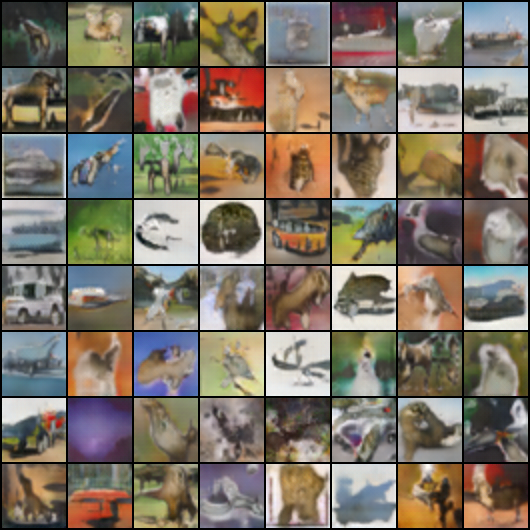
\includegraphics[width=1.0\textwidth]{figures/cifar/192_base_raw_MH.png}
       \caption{MH-GAN}
    \end{subfigure}
    \begin{subfigure}[b]{0.49\textwidth}
       \centering
       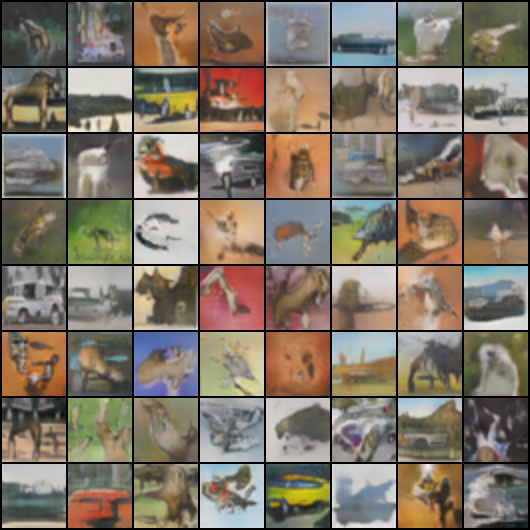
\includegraphics[width=1.0\textwidth]{figures/cifar/192_base_iso_MH.png}
       \caption{MH-GAN (cal)}
    \end{subfigure}
    \caption{{\small
    Example images on CIFAR-10 for different GAN setups.
    The different selectors (MH-GAN and DRS) are run on the same batch of images.
    Meaning, the same images may appear for both generators.
    The calibrated MH-GAN shows a greater preference for animal-like images with four legs.
    }}
    \label{fig:cifar_samples}
\end{figure}


\begin{figure}[htbp]
    \centering
    \begin{subfigure}[b]{0.49\textwidth}
       \centering
       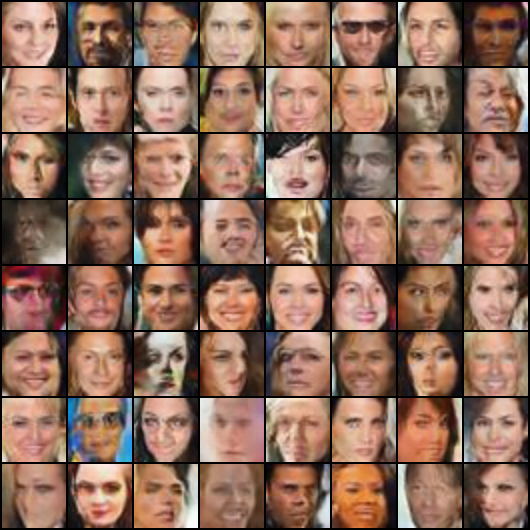
\includegraphics[width=\exfactor\textwidth]{figures/celeba/31_base_raw_base.png}
       \caption{GAN}
    \end{subfigure}
    \begin{subfigure}[b]{0.49\textwidth}
       \centering
       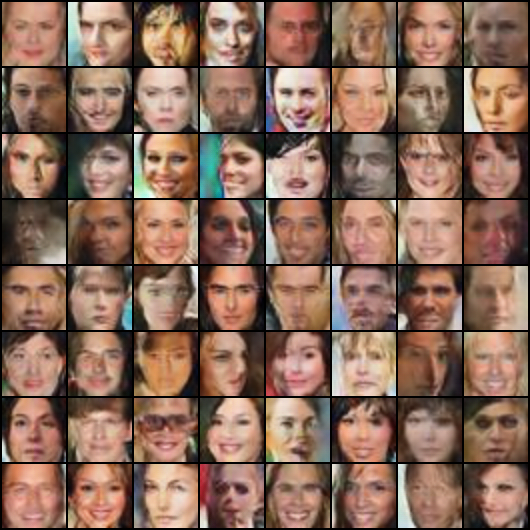
\includegraphics[width=\exfactor\textwidth]{figures/celeba/31_base_raw_reject.png}
       \caption{DRS}
    \end{subfigure}
    \begin{subfigure}[b]{0.49\textwidth}
       \centering
       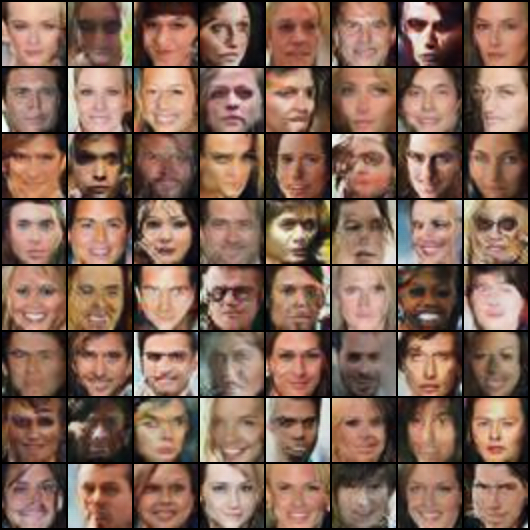
\includegraphics[width=\exfactor\textwidth]{figures/celeba/31_base_raw_MH.png}
       \caption{MH-GAN}
    \end{subfigure}
    \begin{subfigure}[b]{0.49\textwidth}
       \centering
       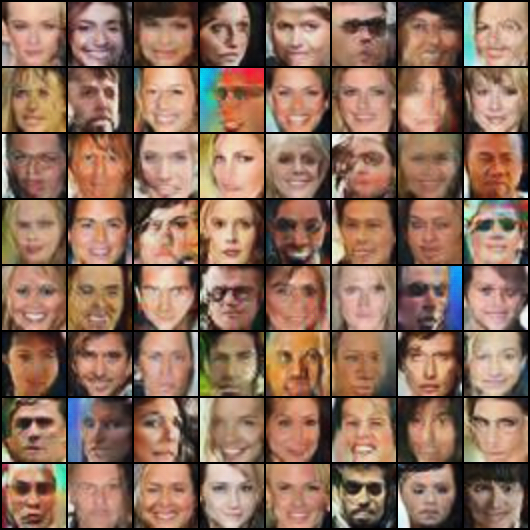
\includegraphics[width=\exfactor\textwidth]{figures/celeba/31_base_iso_MH.png}
       \caption{MH-GAN (cal)}
    \end{subfigure}
    \caption{{\small
    Example images on CelebA for different GAN setups.
    Like Figure~\ref{fig:cifar_samples}, the same batch of images goes into each selector.
    }}
    \label{fig:celeba_samples}
\end{figure}



\end{document}
